\paragraph*{}
In recent years, material classification has become an active topic for reseachers with the main goal is providing the detail of material information for a vareties applications such as Advanced Driver-Assistance Systems (ADAS) \cite{r1}, robotic manipulation \cite{spong2006robot}, robotic navigation \cite{kim2013robot}, etc. 
\begin{figure}[h!]
\centering
\captionsetup{width=0.75\textwidth}
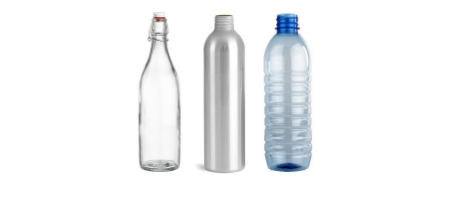
\includegraphics[width=0.7\linewidth]{images/bottles.png}
\caption[An example for where material could be valuable]{Bottles with similary shapes, are made of diffrenet materials which decides its physical properties, which could be extremely useful information in various situations.}
\label{fig:f1}
\end{figure}
\paragraph*{•}
Material of surfaces contribute valuable informations to understand the whole image. For example, Figure \ref{fig:f1} shows that with infomation about material which thoses bottles make of, computer could sort those bottles by weights, make a decision to choose which one is good to hold hot water or even know that it would be a risk to allow people bring a glass bottle which could be used as a weapon into a meeting between head of states.
\paragraph*{}
Previous works on material classification are focused on ... (some previous works here). In this paper, we suggest a ... (summary our work here). 